\section{System Design and Responsibilities}

The Moving Object Pipeline System has two main responsibilities: the
generation and maintenance of the Moving Object database, and the
prediction of known object locations which are sent to the Association
Pipeline to prevent unneccessary alerts.  The MOPS has been broken
into two components, colloquially known as ``DayMOPS'' and ``NightMOPS.''
Both are based on designs and algorithms in use in the PanSTARRS MOPS
system.
 

\begin{figure}[!ht]
\centering
  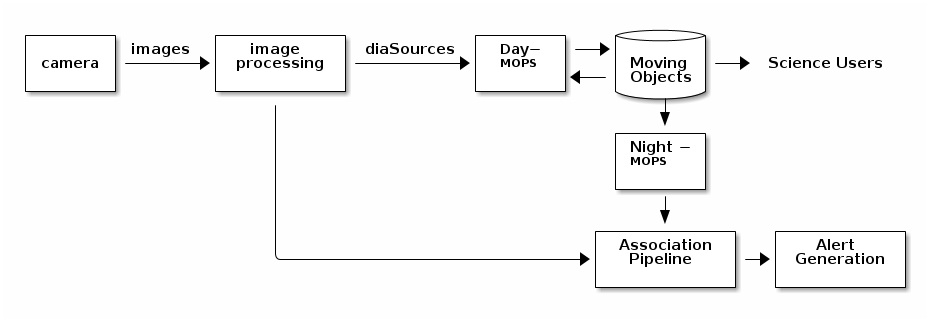
\includegraphics[width=13cm]{illustrations/mopsWithinLsst.png}
\caption{ Data flow from the camera through DayMOPS to the Science
  Users and Alert Generation.  DayMOPS will build and maintain the
  Moving Objects table, NightMOPS will use the Moving Objects table to
  communicate with the Assocation Pipeline.  }
\label{mopsWithinLsst}
\end{figure}


``DayMOPS,'' so called because it processes data acquired from the
previous night in a large batch operation, is responsible for
discovering new Moving Objects in newly-acquired data, searching old
data for detections of new objects, and updating the Moving Objects
table to reflect newly-acquired data. It is also responsible for
periodically cleaning and refining the contents of the Moving Objects
table.  ``NightMOPS'' is responsible for projecting the locations of known
Moving Objects in upcoming images as they are announced during
night-time operations.  

The relationship between DayMOPS, NightMOPS and the neighboring
components of the LSST Data Management system is illustrated in
figure \ref{mopsWithinLsst}.

\subsection{DayMOPS: Discovering and Managing Moving Objects}

% Illustration of DayMOPS

% sky-plane vs. orbit-space illustration

The DayMOPS is responsible for discovering moving objects in source
catalogs.  The task of discovering and tracking asteroids has been
performed by humans since hundreds of years ago, but automated systems
for asteroid discovery and tracking remain relatively uncommon.  Other
surveys have often mixed human and computerized approaches -
\textbf{can we get some more history here?}.


For the LSST DayMOPS, we have chosen to follow the model of the
PanSTARRS Moving Object Pipeline System \citep{psMOPSDesign}.  The
approach used here is to first find sets of detections with sky-plane
paths consistent with asteroid behaviour; these sets of detections and
their fitted paths are called \textbf{tracks}.  A set of algorithms
for the discovery of sky-plane tracks in dense data are presented in
\citet{Kubica:2005:MTA:1081870.1081889}; these algorithms are used in
the PanSTARRS MOPS and the basis of the linking methods for the
current LSST DayMOPS.  

The tracking methods used are based on a tiered approach; first two or
more detections from a single night are linked into
\textbf{tracklets}, which represent a hypothetical object and a linear
approximation of its sky-plane motion.  These tracklets are later
joined into larger tracks.  To suit the needs of orbit fitting, we are
generally only interested in tracks containing tracklets from at least
three nights, and because of the increasing complexity of sky-plane
motion over time, we are generally interested in tracks which span no
more than 15-30 days of observation time.

The PanSTARRS MOPS uses a fairly loose and generous approximation of
asteroid motion.  This allows for many mislinkages or \textbf{false
  tracks}, combining detections which are not attributable to the same
source, but virtually all objects for which a true (correctly-linked)
track could be generated will get some correct track.  With LSST's
expected density of detections, we found that this glut of false
tracks was generally too painful.  As a result, our methods diverge
from those of PanSTARRS as we introduce some more strict filters on
tracks, reducing the number of mislinkages at the expense of
potentially missing some true tracks.  The algorithms, their
implementations, the additional filters, and their behaviors are
presented thoroughly in Chapter \ref{linking}.

Once tracks are discovered, they are sent to the Orbit Determination
phase. The Orbit Determination phase takes these sets of sky-plane
detections and attempts to find a Keplerian orbit which could generate
the detections.  This orbit is further refined, and error bounds are
established, using differential correction.  Orbit Determination will
reject many tracks as false, but should successfully find precise
orbits for virtually all correctly linked tracks.  Several methods for
performing this task are known, and several have open-source implementations
available to LSST \citep{Milani04orbitdetermination},
\citep{Milani2006}, \citep{OpenOrb2009}, \citep{granvik_thesis}.  The
orbits discovered by Orbit Determination, and the detections present
in the track associated with each orbit, are used to generate new
Moving Objects.

\begin{figure}[h]
\begin{center}
  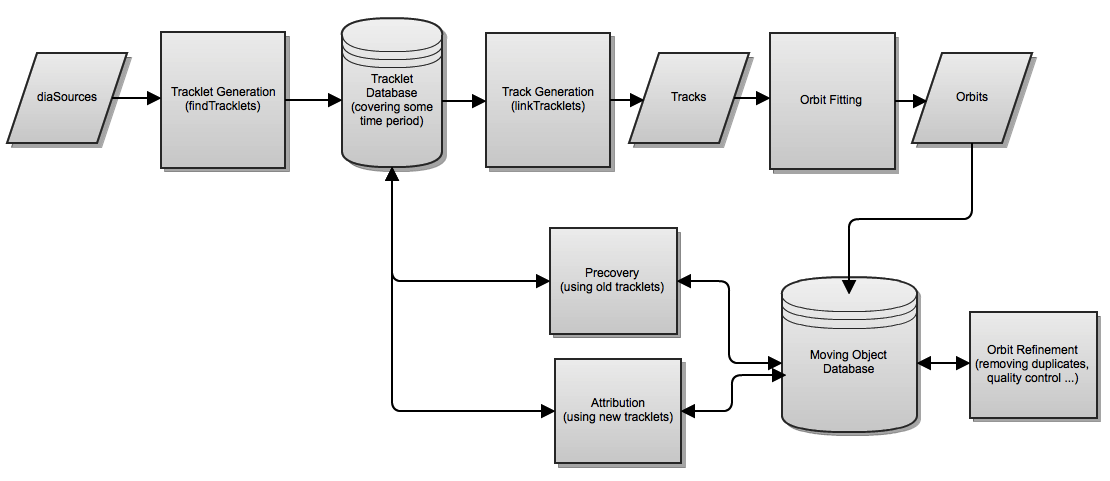
\includegraphics[width=11cm]{illustrations/mopsDiagram.png}
\end{center}
\caption{ Data flows into the DayMOPS pipeline and results in
  modifications of the Moving Objects table in a variety of ways,
  including attribution to known objects, a multi-stage pipeline for
  the discovery of new objects, and periodic refinements of the Moving
  Object table, such as possible merges of redundant objects or
  removal of false orbits. }
\label{mopsDiagram}
\end{figure}



As in the PanSTARRS MOPS design \citep{psMOPSDesign} the LSST's
DayMOPS is expected to perform several additional tasks to manage and
improve the Moving Objects table over time.  Attribution is the
process of identifying known objects in incoming data and adding those
detections to the correct Moving Object (this task is delegated to
NightMOPS). Similarly, Precovery is the recovery of known,
unattributed detections associated with a newly-discovered Moving
Object.  Another refinement is the merging of potentially redundant
Moving Objects.  The complete set of DayMOPS tasks and their data
flows are illustrated in figure \ref{mopsDiagram}.









\subsection{NightMOPS: Predicting Moving Object Locations}

The NightMOPS section of MOPS is responsible for predicting the
locations of known Moving Objects as images are taken, so that they
may be attributed to the known Moving Objects and removed from the set
of unknown transients detections.  This allows attribution for known
Moving Objects, improving the quality of the Moving Object data
products, and also allows the prevention of unnecessary Alerts.

Predicting the locations of objects given an orbit can be accomplished
through ephemeris calculation using existing orbit-space software
suites \citep{Milani2006}, \citep{OpenOrb2009}.  However, ephemeris
calculation can be fairly slow for large data sets.  Because the
observations schedule for LSST will be determined dynamically, it is
necessary to generate ephemeris predictions for a potentially large
Moving Object table in a short period of time.

% some kind of time-domain illustration?

In order to accomplish this, NightMOPS will generate ``coarse
ephemerides'' for known objects, predicting their locations at the
beginning and end of the night.  Then, when given an upcoming image
location, NightMOPS will use interpolation of the coarse ephemerides
to find objects which could feasibly be present in the upcoming
image. Precise ephemerides for just these objects will be
generated. In this way, NightMOPS will avoid the problem of generating
ephemeris for each known Moving Object for every image time.


\subsection{Implementation Status}

All software components of MOPS, with the possible exception of
initial orbit determination, differential correction, and ephemeris
generation, are expected to be completed in open-source C++ compliant
with LSST software guidelines and in LSST appropriate coding style.
These components will run inside the LSST Pipeline Framework.

Currently, the initial tracking phases of DayMOPS are implemented in
LSST-compliant C++.  The selection of an appropriate package for
initial orbit determination, orbital differential correction, and
ephemeris generation is incomplete but several FORTRAN options are
available to us, some open-source \citep{Milani2006}
\citep{OpenOrb2009}.  A Python-based implementation of NightMOPS,
using the LSST Pipeline Framework, is complete but it is currently
using a closed-source ephemeris generation tool.

